\section[Realization in terms of q-Weyl algebras]{Realization in terms of $\boldsymbol{q}$-Weyl algebras}\label{s:qw}

\subsection[Y-variables and q-Weyl algebras]{$\boldsymbol{Y}$-variables and $\boldsymbol{q}$-Weyl algebras}

Hereafter we also use $\hbar $ which is related to $q$ by
$q=\e^\hbar$. By a $q$-Weyl algebra we mean an associative algebra
generated by $U^{\pm 1}$ and $W^{\pm 1}$ obeying the relations
$U U^{-1} = U^{-1} U= W W^{-1} = W^{-1}W = 1$ and $UW = q WU$.
%
To each crossing $i$ of the wiring diagram we associate parameters~${\mathscr{P}_i = (a_i, b_i, c_i, d_i, e_i)}$ and canonical variables
$\uu_i$, $\ww_i$ satisfying
\begin{align}
&[\uu_i, \ww_j]= \hbar \delta_{ij}, \qquad [\uu_i, \uu_j]=[\ww_i, \ww_j]=0.
\label{uwh}
\\
&a_i+b_i+c_i+d_i+e_i=0.
\label{ae0}
\end{align}
The exponentials of the canonical variables obey the relations in a
direct product of $q$-Weyl algebras, e.g.,
$\e^{\uu_i} \e^{\ww_j} = q^{\delta_{ij}}\e^{\ww_j}\e^{\uu_i}$. Given a wiring
diagram and the associated symmetric butterfly quiver, we
``parametrize'' the $Y$-variables by the graphical rule explained in
Figure~\ref{fig:para}.

\begin{figure}[t]\centering
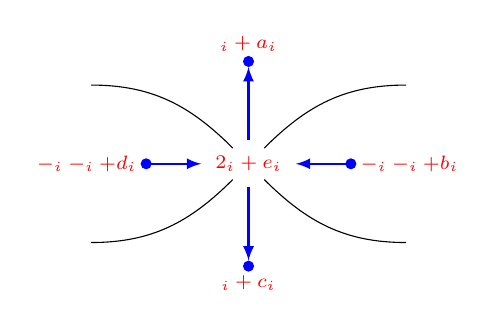
\begin{tikzpicture}
\begin{scope}[>=latex,xshift=0pt]
\draw [-] (0,2) to [out = 0, in = 135] (1.8,1.2);
\draw [-] (0,0) to [out = 0, in = -135] (1.8,0.8);
\draw [-] (2.2,0.8) to [out = -45, in = 180] (4,0);
\draw [-] (2.2,1.2) to [out = 45, in = 180] (4,2);
%
{\color{blue}
\fill (0.7,1) circle(2pt) coordinate(A) node[left]{\color{red} \scriptsize{$-\uu_i-\ww_i+d_i$}};
\fill (3.3,1) circle(2pt) coordinate(B) node[right]{\color{red} \scriptsize{$-\uu_i-\ww_i+b_i$}};
\fill (2,2.3) circle(2pt) coordinate(C) node[above]{\color{red} \scriptsize{$\ww_i+a_i$}};
\fill (2,-0.3) circle(2pt) coordinate(D) node[below]{\color{red} \scriptsize{$\ww_i+c_i$}};
\draw (2,1) node {\color{red} \scriptsize{$2\uu_i+e_i$}};
\draw[->,shorten >=2pt] (2,1.3) -- (C) [thick];
\draw[->,shorten >=2pt] (2,0.7) -- (D) [thick];
\draw[->] (A) -- (1.4,1) [thick];
\draw[->] (B) -- (2.6,1) [thick];
\qdarrow{C}{A}
\qdarrow{C}{B}
\qdarrow{D}{A}
\qdarrow{D}{B}
}
\end{scope}
\end{tikzpicture}
\caption{Graphical rule to parametrize the $Y$-variables in terms of
 $q$-Weyl algebra generators in the vicinity of the crossing $i$
 (center) of the wiring diagram (black). A $Y$-variable situated at
 a vertex (blue circle) of the symmetric butterfly quiver acquires
 factors $\e^{a_i+ \ww_i}$, $\e^{b_i-\uu_i-\ww_i}$, $\e^{c_i+\ww_i}$,
 $\e^{d_i-\uu_i-\ww_i}$ from the neighboring crossing $i$ of the wiring
 diagram if the vertex is located at the north, east, south, west of
 $i$, respectively. A $Y$-variable on the vertex $i$ is
 $\e^{e_i+2\uu_i}$. The ordering of these factors from different $i$'s
 (if any) is inconsequential due to the commutativity of the
 associated canonical variables. }\label{fig:para}
\end{figure}


The claim is that the relation
$Y_r Y_s = q^{2b_{rs}}Y_sY_r$ \eqref{yyq} is satisfied under this parametrization.
%
To state it formally, let $\mathcal{W}_n$ be the direct product of the
$q$-Weyl algebras generated by~$\e^{\pm \uu_i}$,~$\e^{\pm \ww_i}$ for
$i=1, \dots, n$. Let further $\mathcal{A}_n$ be the non-commuting
fractional field of $\mathcal{W}_n$. Then for $B$ corresponding to
the left diagram in Figure \ref{fig:R123}, we have a morphism
$\phi_\mathrm{SB}\colon \mathcal{Y}(B) \rightarrow \mathcal{A}_3$
defined by
\begin{align}
\phi_\mathrm{SB}\colon\
\begin{cases}
Y_1 \mapsto \e^{c_1+c_3+\ww_1+\ww_3},
& Y_6 \mapsto \e^{b_1-\uu_1-\ww_1},
\\
Y_2 \mapsto \e^{d_3-\uu_3-\ww_3},
& Y_7 \mapsto \e^{d_2+a_3-\uu_2-\ww_2+\ww_3},
\\
Y_3 \mapsto \e^{e_3+2\uu_3},
& Y_8 \mapsto \e^{e_2+2\uu_2},
\\
Y_4 \mapsto \e^{d_1+c_2+b_3-\uu_1-\ww_1+\ww_2-\uu_3-\ww_3},
& Y_9 \mapsto \e^{a_1+b_2+\ww_1-\uu_2-\ww_2},
\\
Y_5 \mapsto \e^{e_1+2\uu_1},
& Y_{10} \mapsto \e^{a_2+\ww_2},
\end{cases}
\label{Yw}
\end{align}
where SB signifies ``symmetric butterfly''. Similarly, for the right
diagram of Figure \ref{fig:R123}, we have a morphism
$\phi'_\mathrm{SB}\colon \mathcal{Y}\bigl(B'\bigr) \rightarrow \mathcal{A}_3$ as
\begin{align}
\phi'_\mathrm{SB}\colon\
\begin{cases}
Y'_1 \mapsto \e^{c_2+\ww_2},
& Y'_6 \mapsto \e^{b_2+c_3-\uu_2-\ww_2+\ww_3},
\\
Y'_2 \mapsto \e^{c_1+d_2+\ww_1-\uu_2-\ww_2},
& Y'_7 \mapsto \e^{d_1-\uu_1-\ww_1},
\\
Y'_3 \mapsto \e^{e_3+2\uu_3},
& Y'_8 \mapsto \e^{e_2+2\uu_2},
\\
Y'_4 \mapsto \e^{b_1+a_2+d_3-\uu_1-\ww_1+\ww_2-\uu_3-\ww_3},
& Y'_9 \mapsto \e^{b_3-\uu_3-\ww_3},
\\
Y'_5 \mapsto \e^{e_1+2\uu_1},
& Y'_{10} \mapsto \e^{a_1+a_3+\ww_1+\ww_3}.
\end{cases}
\label{Ypw}
\end{align}
